\documentclass{beamer}
\usepackage[utf8]{inputenc}

\usepackage{graphicx}
\graphicspath{{images/}}

\usepackage{tikz}
\usepackage{pgfplots}

\usepackage{hyperref}
\hypersetup{
    colorlinks=true,
    linkcolor=blue,
    filecolor=magenta,
    urlcolor=cyan,
    pdftitle={Overleaf Example},
    pdfpagemode=FullScreen,
    }

\urlstyle{same}

\usetheme{CambridgeUS}
\usecolortheme{default}

%------------------------------------------------------------
%This block of code defines the information to appear in the
%Title page
\title[Beamer sample] %optional
{Homework}

\subtitle{presentation using Beamer}

\author[Tom Choi] % (optional)
{Dongho~(Tom)~Choi\inst{1}}

\institute[UNL] % (optional)
{
  \inst{1}%
  PhD student\\
  Univesrity of Nebraska-Lincoln
}

\date[December 2021] % (optional)
{STAT 850, December 2021}

\logo{\includegraphics[height=1cm]{UNL-logo.jpg}}

%End of title page configuration block
%------------------------------------------------------------



%------------------------------------------------------------
%The next block of commands puts the table of contents at the
%beginning of each section and highlights the current section:

\AtBeginSection[]
{
  \begin{frame}
    \frametitle{Table of Contents}
    \tableofcontents[currentsection]
  \end{frame}
}
%------------------------------------------------------------


\begin{document}

%The next statement creates the title page.
\frame{\titlepage}


%---------------------------------------------------------

\section{Introducing myself}

%---------------------------------------------------------
%Two columns
\begin{frame}
\frametitle{Introducing myself}

\begin{columns}

\column{0.5\textwidth}
Hello! My name is Dongho Choi.
\newline
Please call me Tom.
\newline
\begin{itemize}
\item Doctoral student in Educational psychology
\item Born on Sep. 15th, 1991.
\item Grew up in Wonju, South Korea.
\item \url{https://github.com/tomchoi91}
\end{itemize}

\column{0.5\textwidth}
    \begin{figure}[h]
    \includegraphics[width=0.5\textwidth]{Picture2.png}
    \centering
    \caption{a nice photo}
    \label{fig:photo1}
    \end{figure}
\end{columns}
\end{frame}
%---------------------------------------------------------

\section{My favorite animal}

%---------------------------------------------------------
%Example of the \pause command
\begin{frame}
\frametitle{My favorite animal}
    \begin{figure}[h]
    \includegraphics[width=0.4\textwidth]{cat.jpg}
    \centering
    \caption{a nice cat}
    \label{fig:photo1}
    \end{figure}
\end{frame}
%---------------------------------------------------------

\section{My favorite plot}

%---------------------------------------------------------
%Highlighting text
\begin{frame}
\frametitle{My favorite plot}
    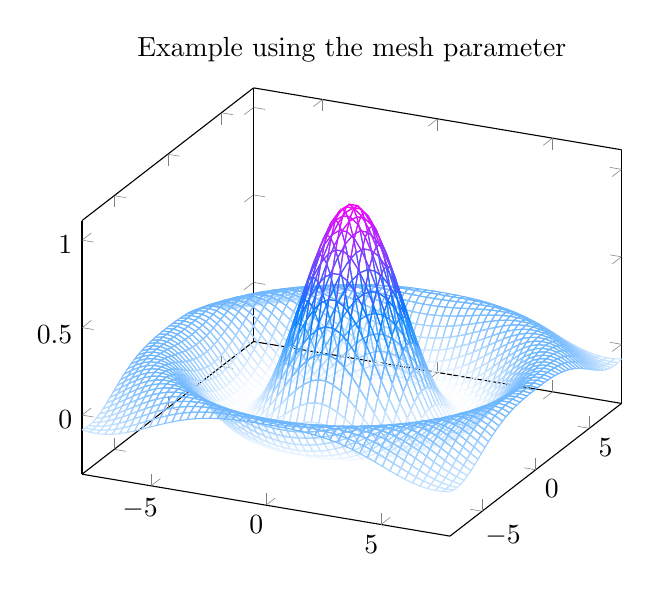
\begin{tikzpicture}
        \begin{axis}[
            title=Example using the mesh parameter,
            % hide axis,
            colormap/cool,
        ]
        \addplot3[
            mesh,
            samples=50,
            domain=-8:8,
        ]
        {sin(deg(sqrt(x^2+y^2)))/sqrt(x^2+y^2)};

        \end{axis}
    \end{tikzpicture}

\end{frame}
%---------------------------------------------------------

\section{My CV}

%---------------------------------------------------------
%Two columns
\begin{frame}
\frametitle{My CV}

please check my \href{https://tomchoi91.github.io/CV/CV_CHOI_TOM.html}{CV}

\end{frame}
%---------------------------------------------------------


\end{document}
